%% $Id: smr-urbansim.tex,v 1.3 2007/05/21 06:28:09 pwaddell Exp $

\documentclass[12pt,a4paper]{article}

\usepackage{txfonts}
\usepackage[T1]{fontenc}
%\usepackage[latin1]{inputenc}

\usepackage{array}
%\usepackage{lscape}
\usepackage{rotating}
\usepackage{longtable}
\usepackage{lscape}
%\usepackage{natbib}
\usepackage{url}
\usepackage{graphics,graphicx}
\usepackage{supertabular}

%
% Change coordinates to edge of page
\voffset=-1in \hoffset=-1in
%
% Set for US Letter
\textheight=9.5in \textwidth=6.5in \topmargin=0.5in
\oddsidemargin=1in \evensidemargin=1in
%
\frenchspacing \raggedbottom
%\renewcommand{\thesection}{\Alph{section}}
%\renewcommand{\theenumii}{\arabic{enumii}}

%\newcommand{\ve}[1]{\mathbf{#1}}
\newcommand{\vk}[1]{\mbox{\boldmath $#1$}}
\newcommand{\tight}{\itemsep 0pt}

\begin{document}

\title{Modeling Household Residential Location Choices and Neighborhood Composition}

\author{\\
%Paul Waddell\\
%Evans School of Public Affairs, University of Washington,\\
%Box 353055, Seattle, WA 98195 \\
%( 206) 221-4161, pwaddell@u.washington.edu
}\maketitle


\baselineskip=.3in

\begin{abstract}
\baselineskip=.3in

The choice of residential location by individual households
determines many aspects of the quality of the social, economic and
physical environment experienced by its members, and there are
well-documented adverse effects of living in neighborhoods with
high concentrations of poor and racial minorities.  We seek to
analyze the processes of household choice of residential location,
and the neighborhood dynamics that emerge from these individual
choices.  Unfortunately, analysis of this choice process is
complicated by the endogeneity of neighborhood social composition,
housing prices, housing supply, and even of the spatial pattern of
access to employment. This paper describes an effort to gain new
analytical insights into the relationships between individual
household choices and emergent outcomes by developing disaggregate
discrete choice models and linking them in an agent-based
simulation system. The framework is developed and applied to data
from the Seattle metropolitan area, using a new open-source
simulation platform and incorporating endogenous processes of
residential location, housing supply, prices, job location, and
travel.  We conclude with a description of a new Open Platform
for Urban Simulation, an Open Source software system for specifying, 
estimating, simulating and visualizing models of urban spatial
dynamics.

\end{abstract}
\clearpage

\section{Introduction}
Problems associated with neighborhood racial segregation and
concentration of poverty, and the dynamic processes of neighborhood
decline, and at times revitalization or gentrification, have been
the subject of sustained academic research from various social
science perspectives for decades. Yet significant issues remain
difficult to address in this research domain, which lies at the
intersection between microscopic perspectives that focus on
individual choices such as residential location, and macroscopic
perspectives that focus on the aggregate dynamics and emergent
spatial patterns across neighborhoods.  The extensive research
assessing neighborhood effects on individual outcomes such as
employment or dropping out of high-school attempts to link these
micro and macro perspectives by examining how the neighborhood
context shapes individual experiences.  There is relatively little
research, on the other hand, that attempts to explore neighborhood
dynamics by analyzing the dynamic choices of individuals.

The issues of neighborhood segregation and dynamics lie at the
intersection of several lines of research that have emerged over the
past three decades, including work on the urban underclass
\cite{wilson-book-1987}, the suburbanization of employment
opportunities and the resulting 'spatial mismatch' of jobs and
inner-city poor blacks \cite{kain-qje-1968}, economic restructuring
that is eliminating high paying manufacturing jobs in the central
city and creating high paying knowledge sector and low paying
service jobs \cite{kasarda-1985}, the filtering of housing from
higher to lower socioeconomic levels producing abandonment in the
poorest inner-city neighborhoods \cite{stegman-aereuea-1977}, racial
preferences in residential location \cite{clark-demography-1992},
increasing racial and economic segregation until 1990
\cite{jargowsky-asr-1996,jargowsky-book-1997,massey-ajs-1990}, and a
significant decline in poverty concentration between 1990 and 2000
\cite{jargowsky-brookings-2003}. The adverse consequences of living
in poor neighborhoods have received substantial attention in the
literature following Wilson's \cite{wilson-book-1987} argument that
concentrated male black joblessness isolates ghetto residents from
the world of work, and promotes a culture of dependency.

Data from the Seattle-Tacoma metropolitan area from the decennial
censuses of 1970 - 2000, mapped in Figure 1 reveal similar dynamics
to those documented by Jargowsky \cite{jargowsky-asr-1996} for a
variety of metropolitan areas, with historically very central and
concentrated pockets of high poverty gradually expanding as nearby
census tracts increase in poverty rate from 1970 to 1990, with
significant retrenchment by 2000. Somewhat similar dynamics occurred
with respect to the segregation of blacks as shown in Figure 2, with
a very high concentration in a few tightly clustered census tracts
in 1970 gradually expanding, following the outward movement of
blacks and the more rapid outmigration of whites. Unlike the poverty
concentration dynamics, however, no prominent decreases in
percentage black appear after 1990, indicating that even as poverty
abated somewhat during the 1990s, racial segregation in the most
segregated neighborhoods did not. Over the same time, there is a
visible dispersion of poor and black populations into neighborhoods
far from their earlier concentrations, both within the central city
and in the suburbs.

\begin{figure}[h]
\centerline{
 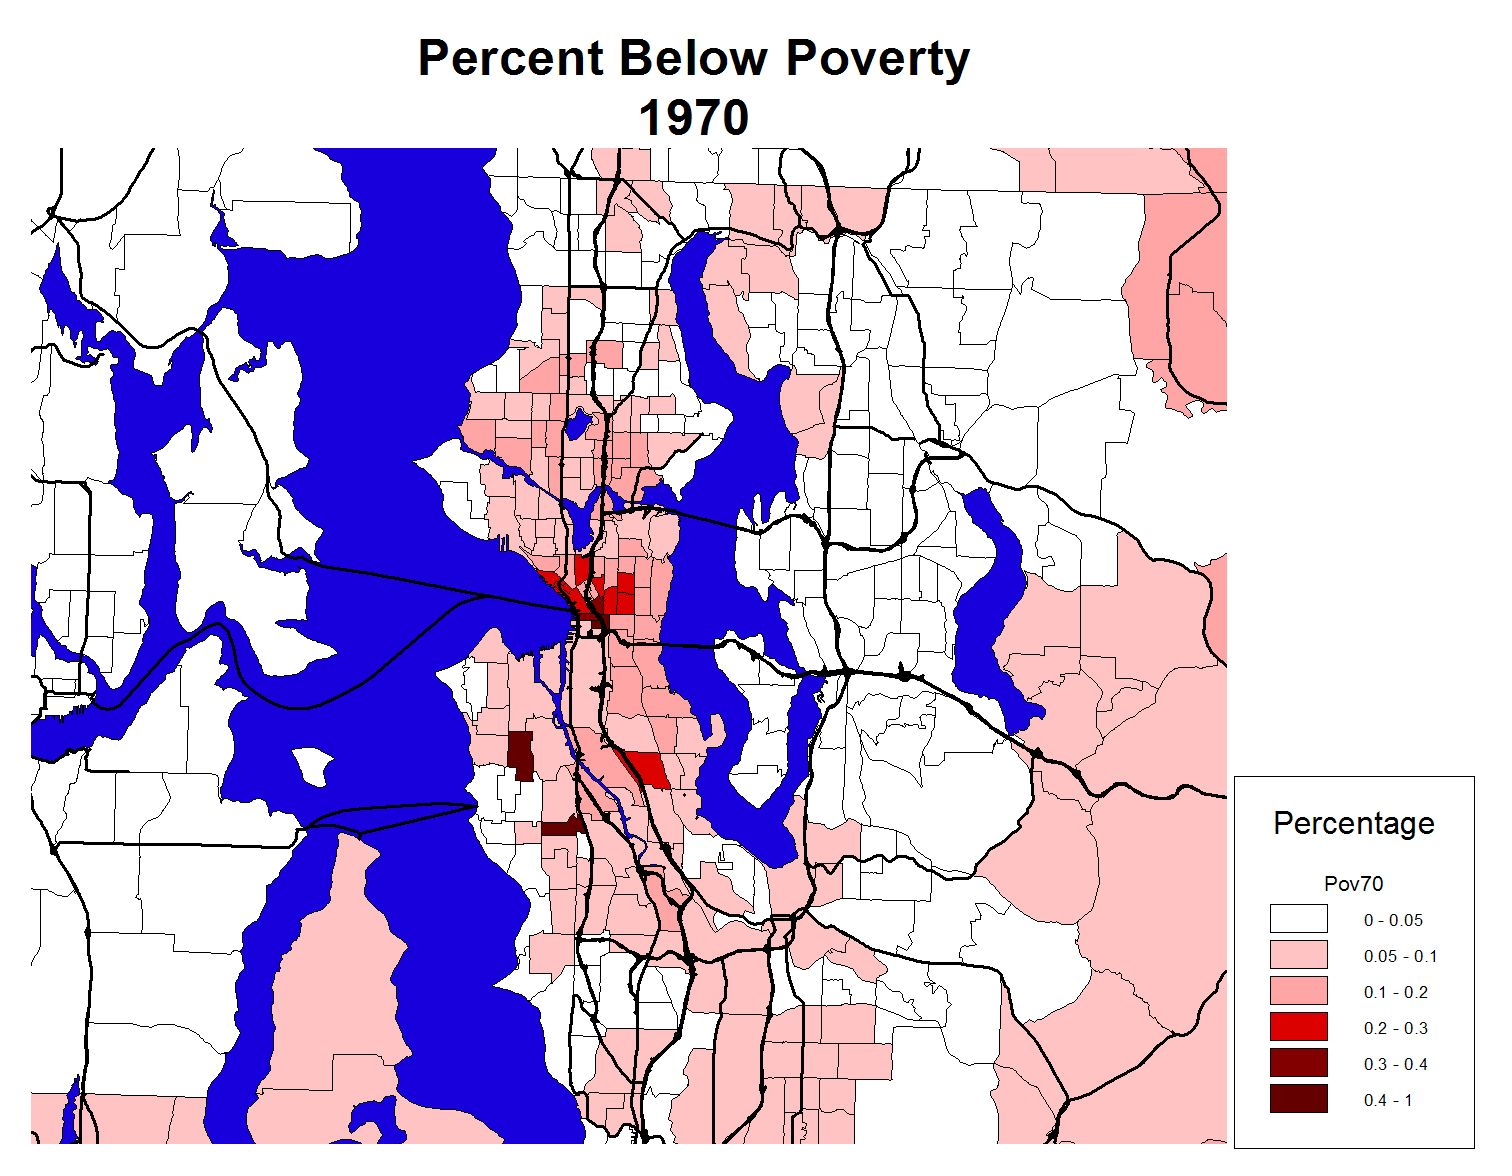
\includegraphics[width=.45\textwidth,height=0.35\textwidth]
 {pctpoor1970.jpg} \hspace{1cm}
 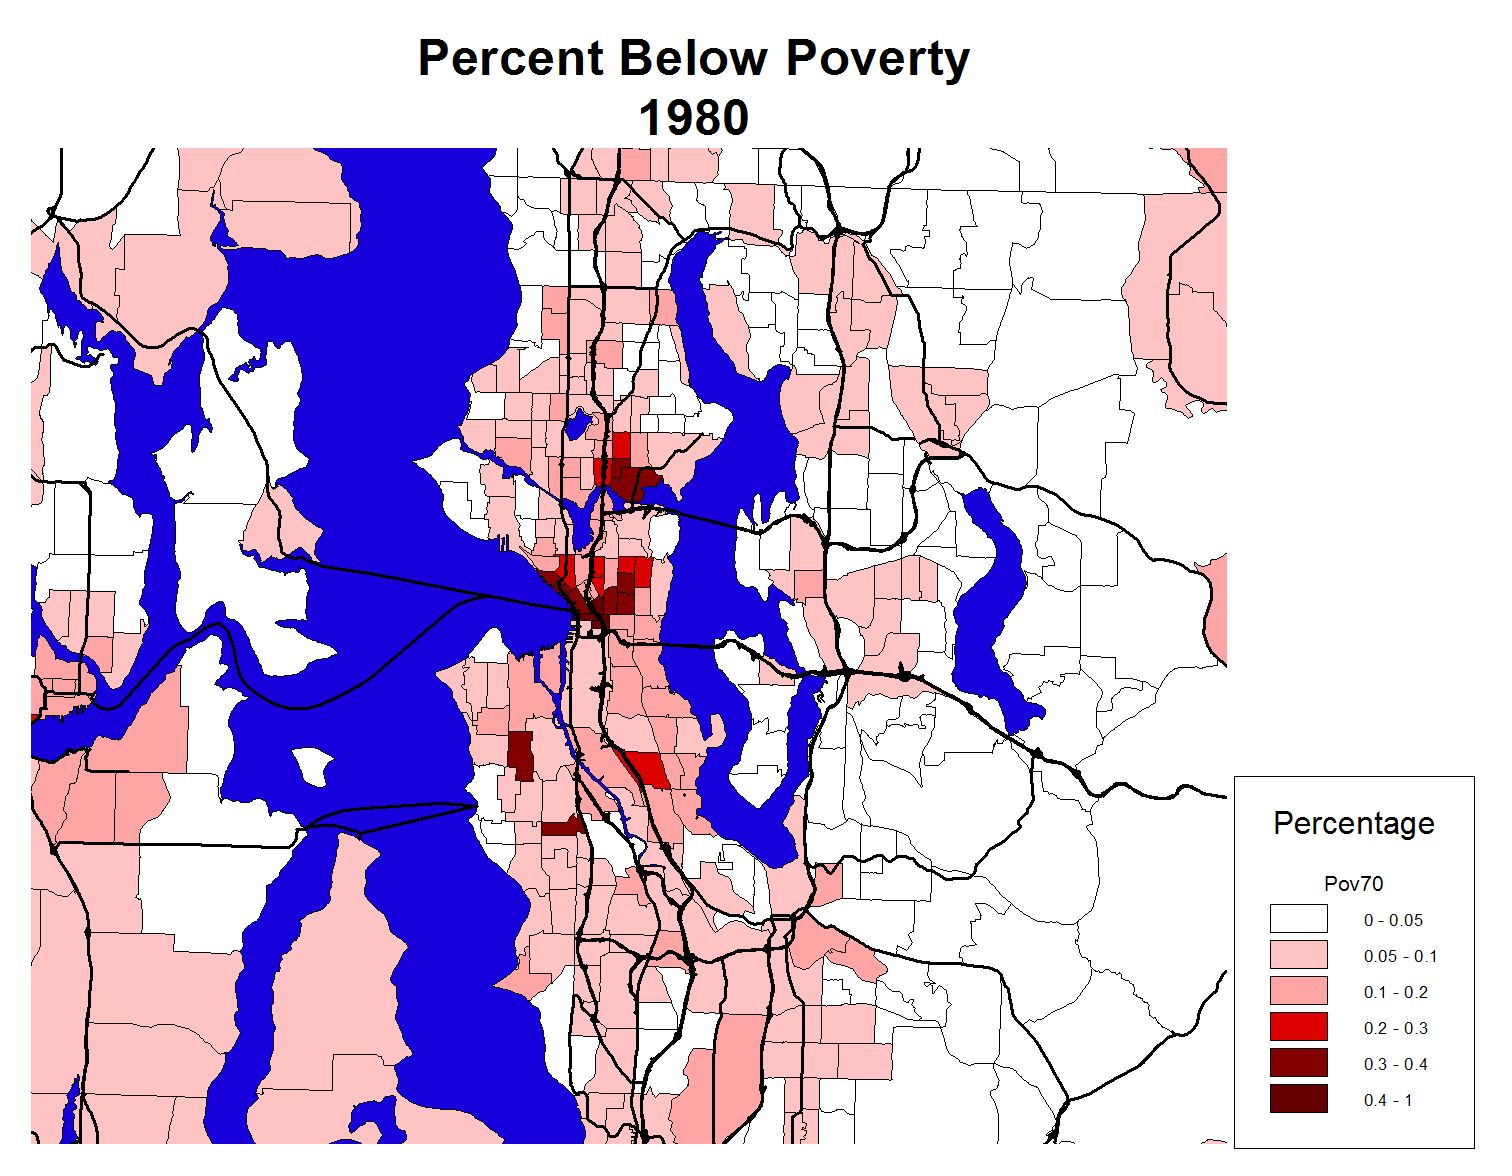
\includegraphics[width=.45\textwidth,height=0.35\textwidth]
 {pctpoor1980.jpg}}
\end{figure}

\begin{figure}[h]
\centerline{
 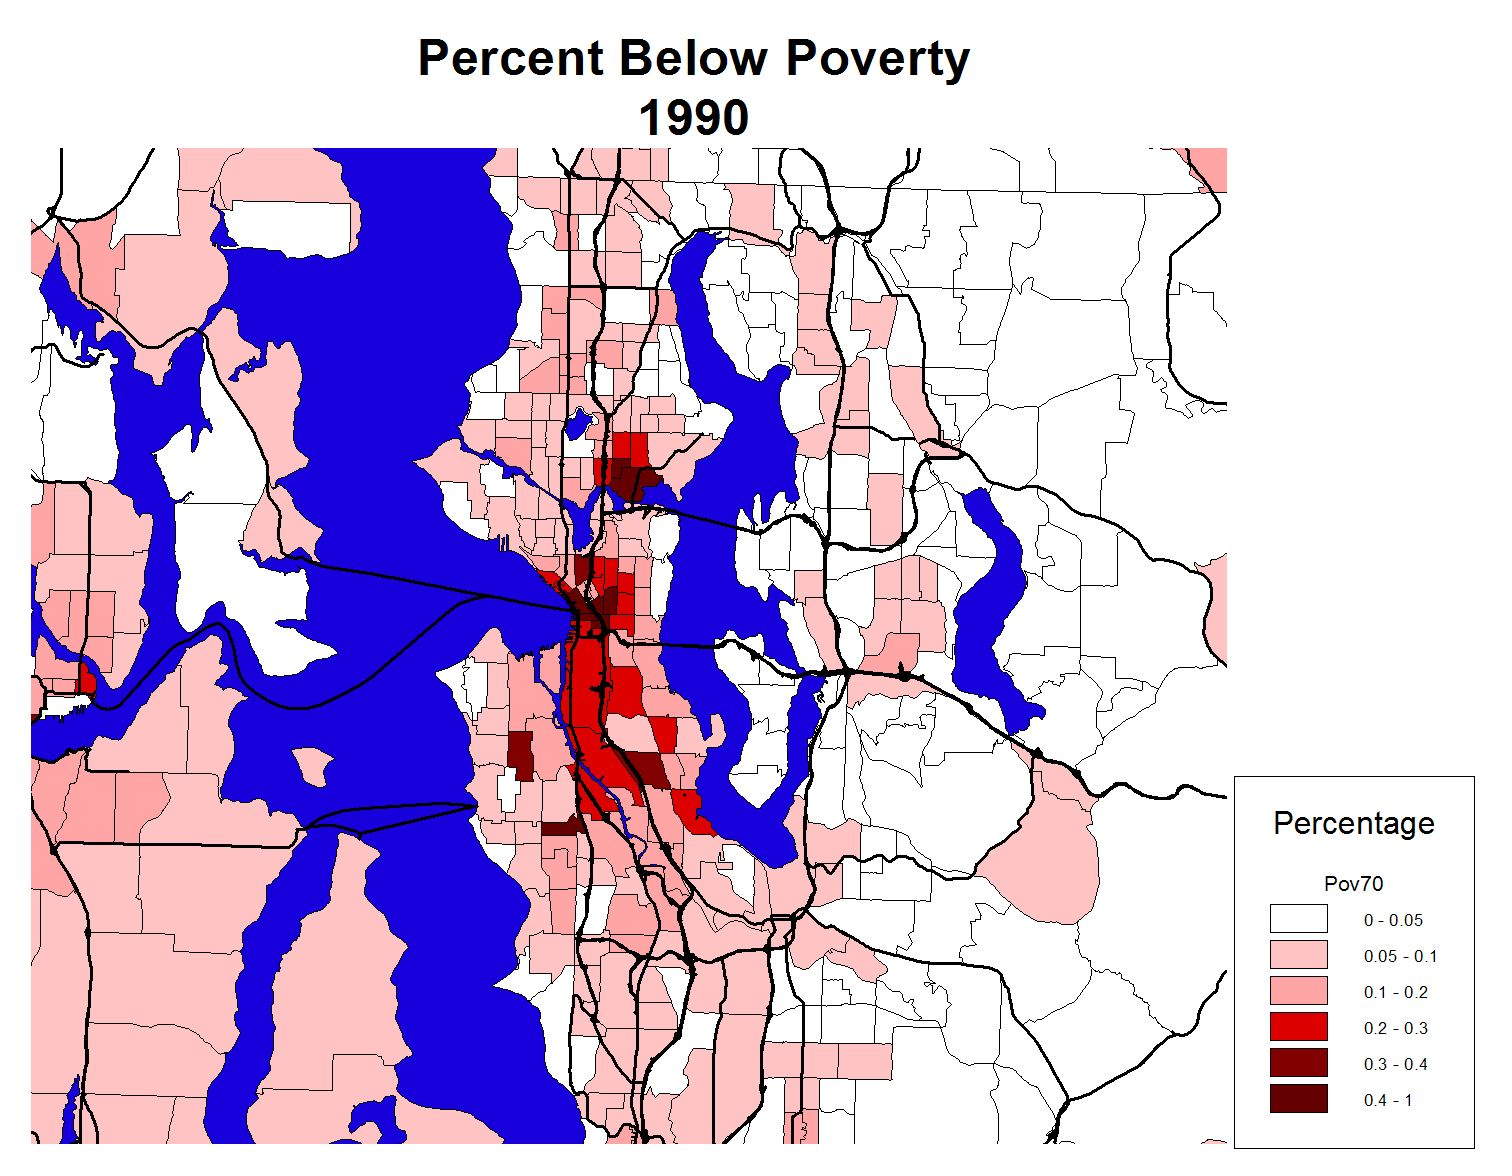
\includegraphics[width=.45\textwidth,height=0.35\textwidth]
 {pctpoor1990.jpg} \hspace{1cm}
 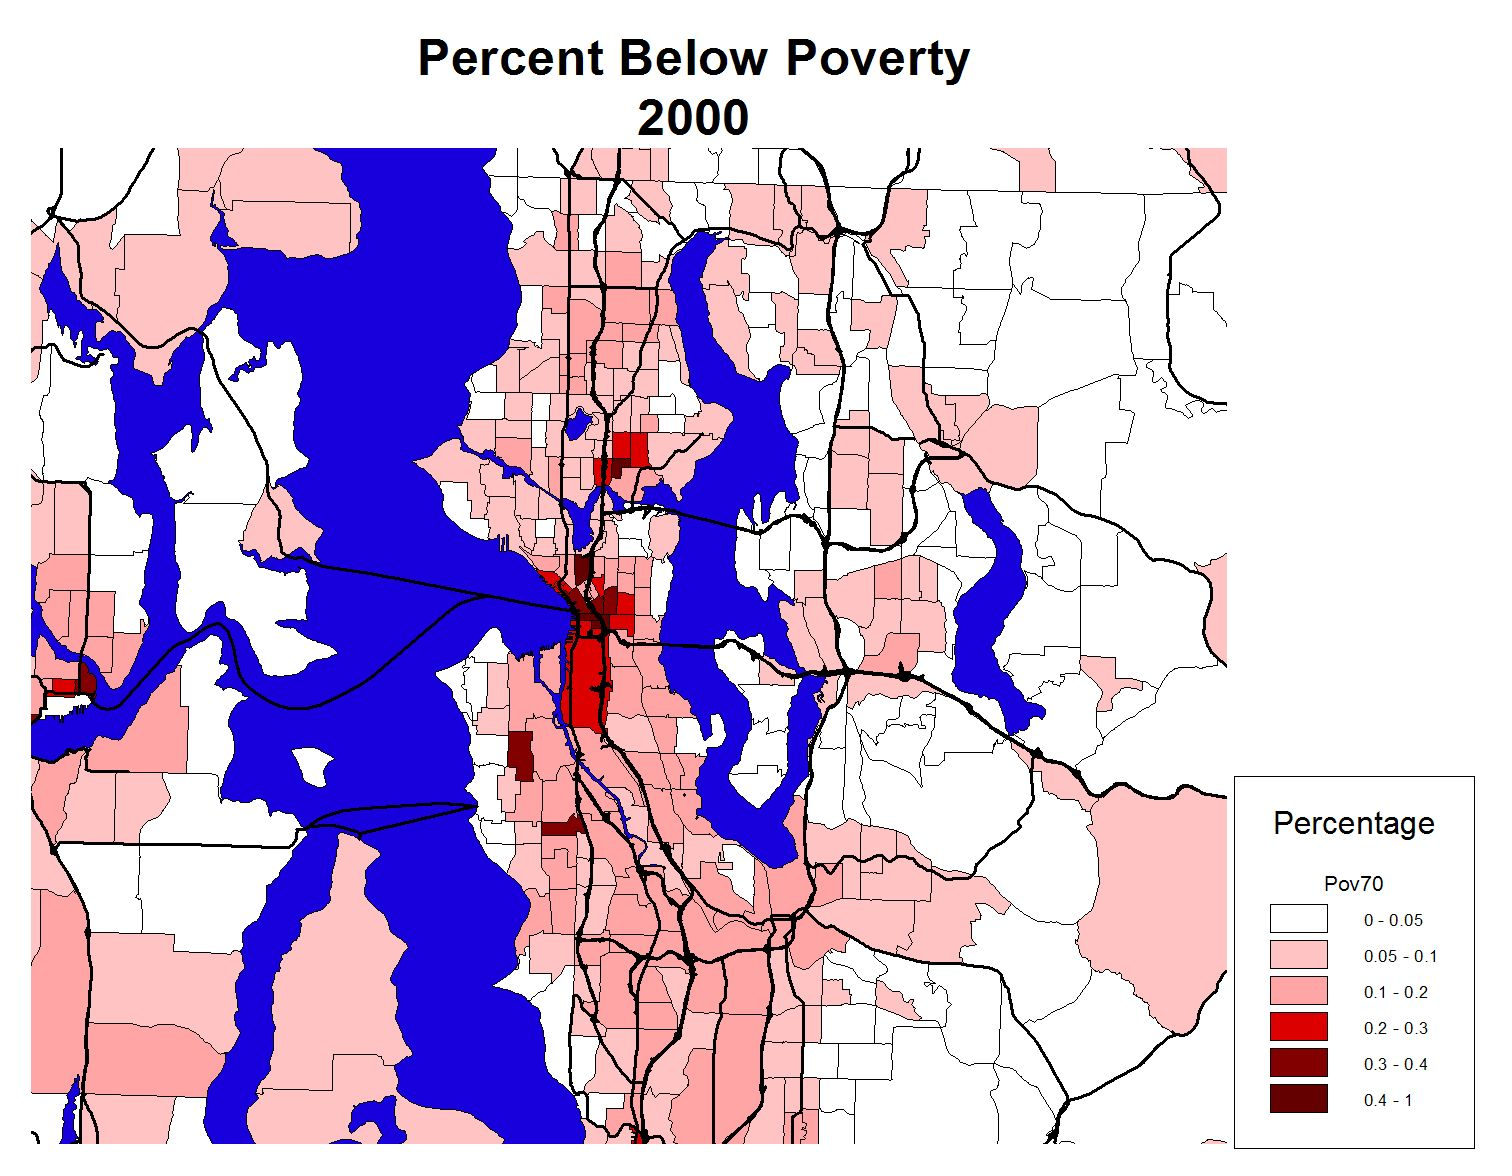
\includegraphics[width=.45\textwidth,height=0.35\textwidth]
 {pctpoor2000.jpg}}
\caption{\label{fig:pctpoor} Percent Poor in Central Seattle}
\end{figure}

These neighborhood dynamics are the result of many interacting
decisions and circumstances, and are therefore difficult to
analyze in the aggregate.  These qualitative images might lend
support to the hypothesis that there are significant differences
in preferences between whites and blacks for locating in highly
segregated neighborhoods, with whites showing stronger aversion to
neighborhoods with a sizable non-white population, and some
reluctance by whites to move into neighborhoods once the
percentage non-white reaches a certain threshold.  There is slight
qualitative support for a parallel hypothesis that similar
preferences occur with respect to the poverty rate in a
neighborhood, though the post-1990 trend appears counter to this.
The maps and the aggregate data they represent, however, cannot
ultimately reveal much about the nature of the preferences of the
households who chose to move out of and into these neighborhoods,
and it would be an ecological fallacy to attribute to individuals
any specific behavior from these aggregate observations. These
data do not, for example, tell us much about how the availability
and price of housing influenced these outcomes, or how the spatial
distribution of jobs and the accessibility provided by the
transport system shaped these choices.  These limitations are the
challenges that motivate this paper.

\begin{figure}[h]
\centerline{
 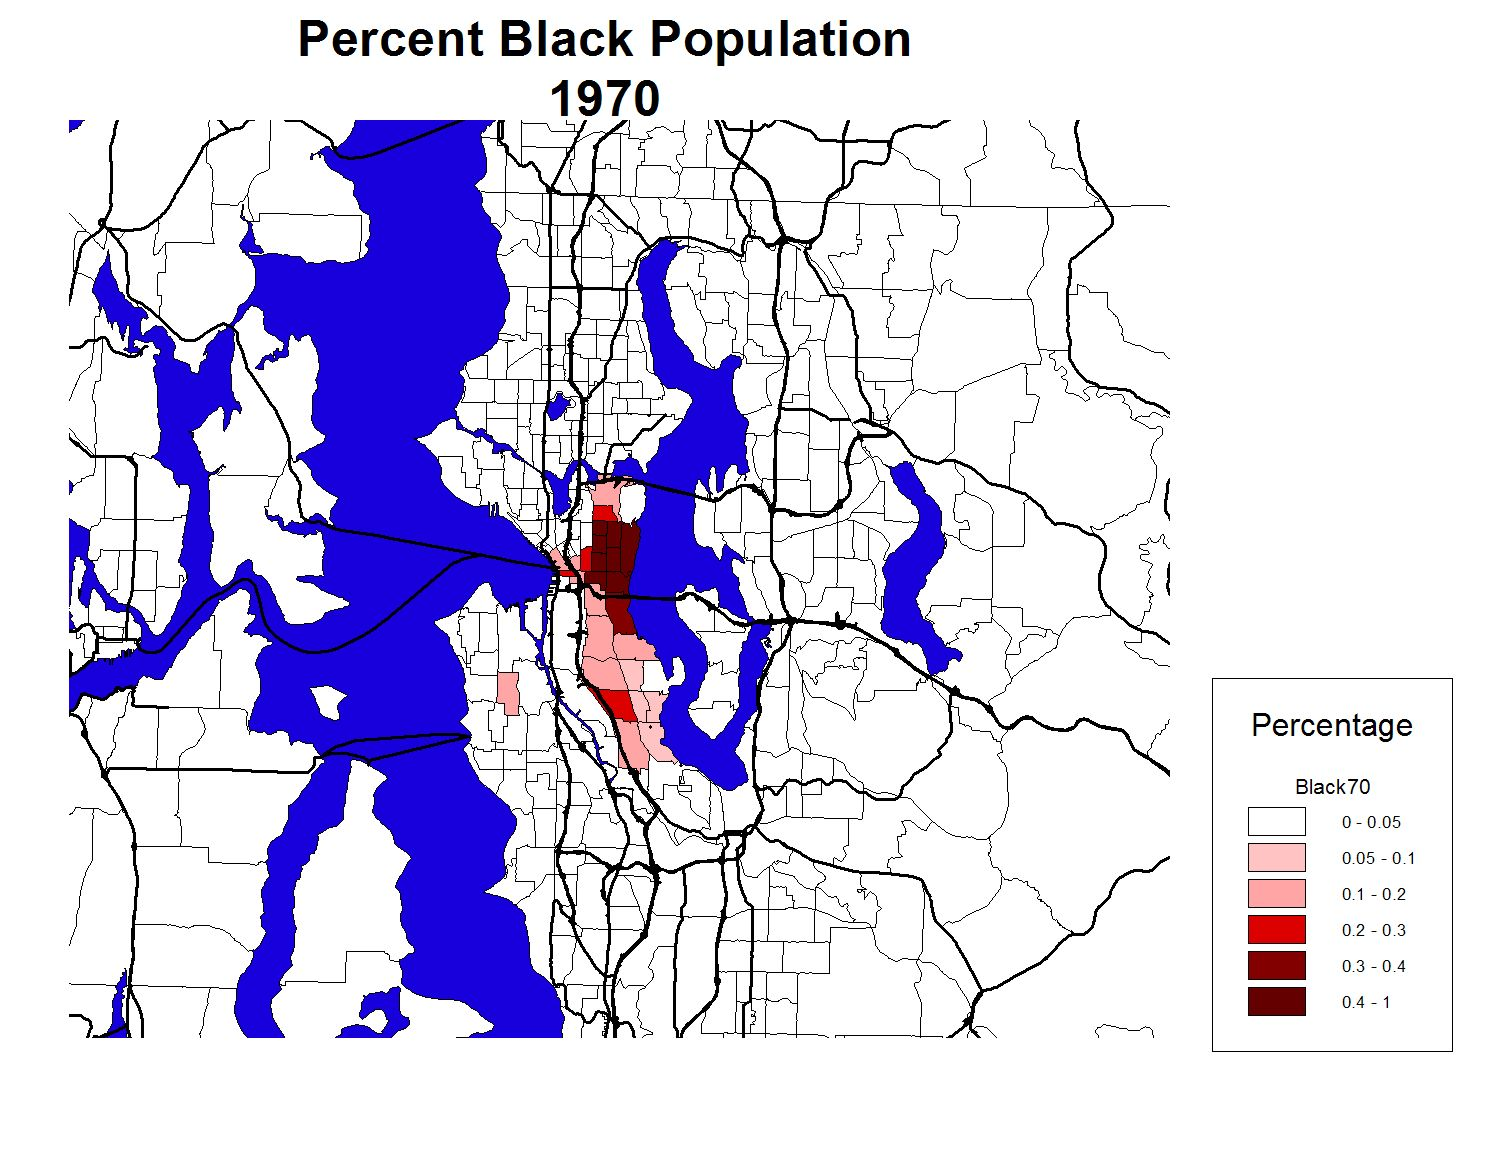
\includegraphics[width=.45\textwidth,height=0.35\textwidth]
 {pctblack1970.jpg} \hspace{1cm}
 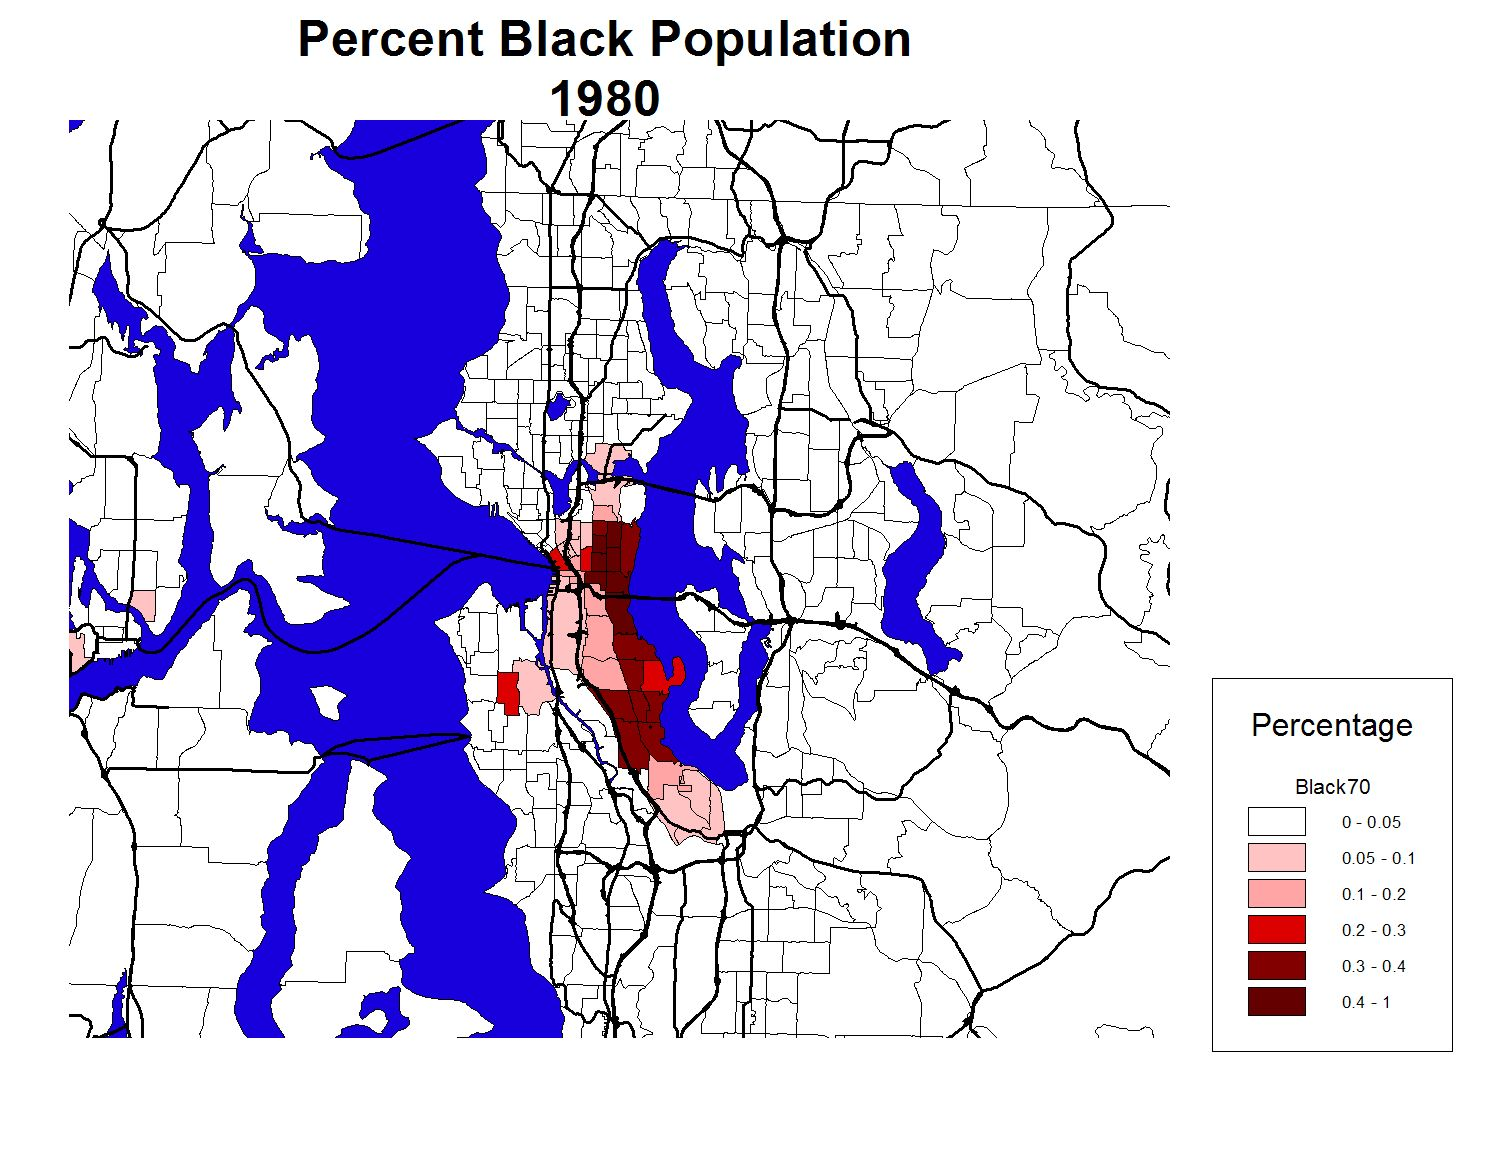
\includegraphics[width=.45\textwidth,height=0.35\textwidth]
 {pctblack1980.jpg}}
\end{figure}

\begin{figure}[h]
\centerline{
 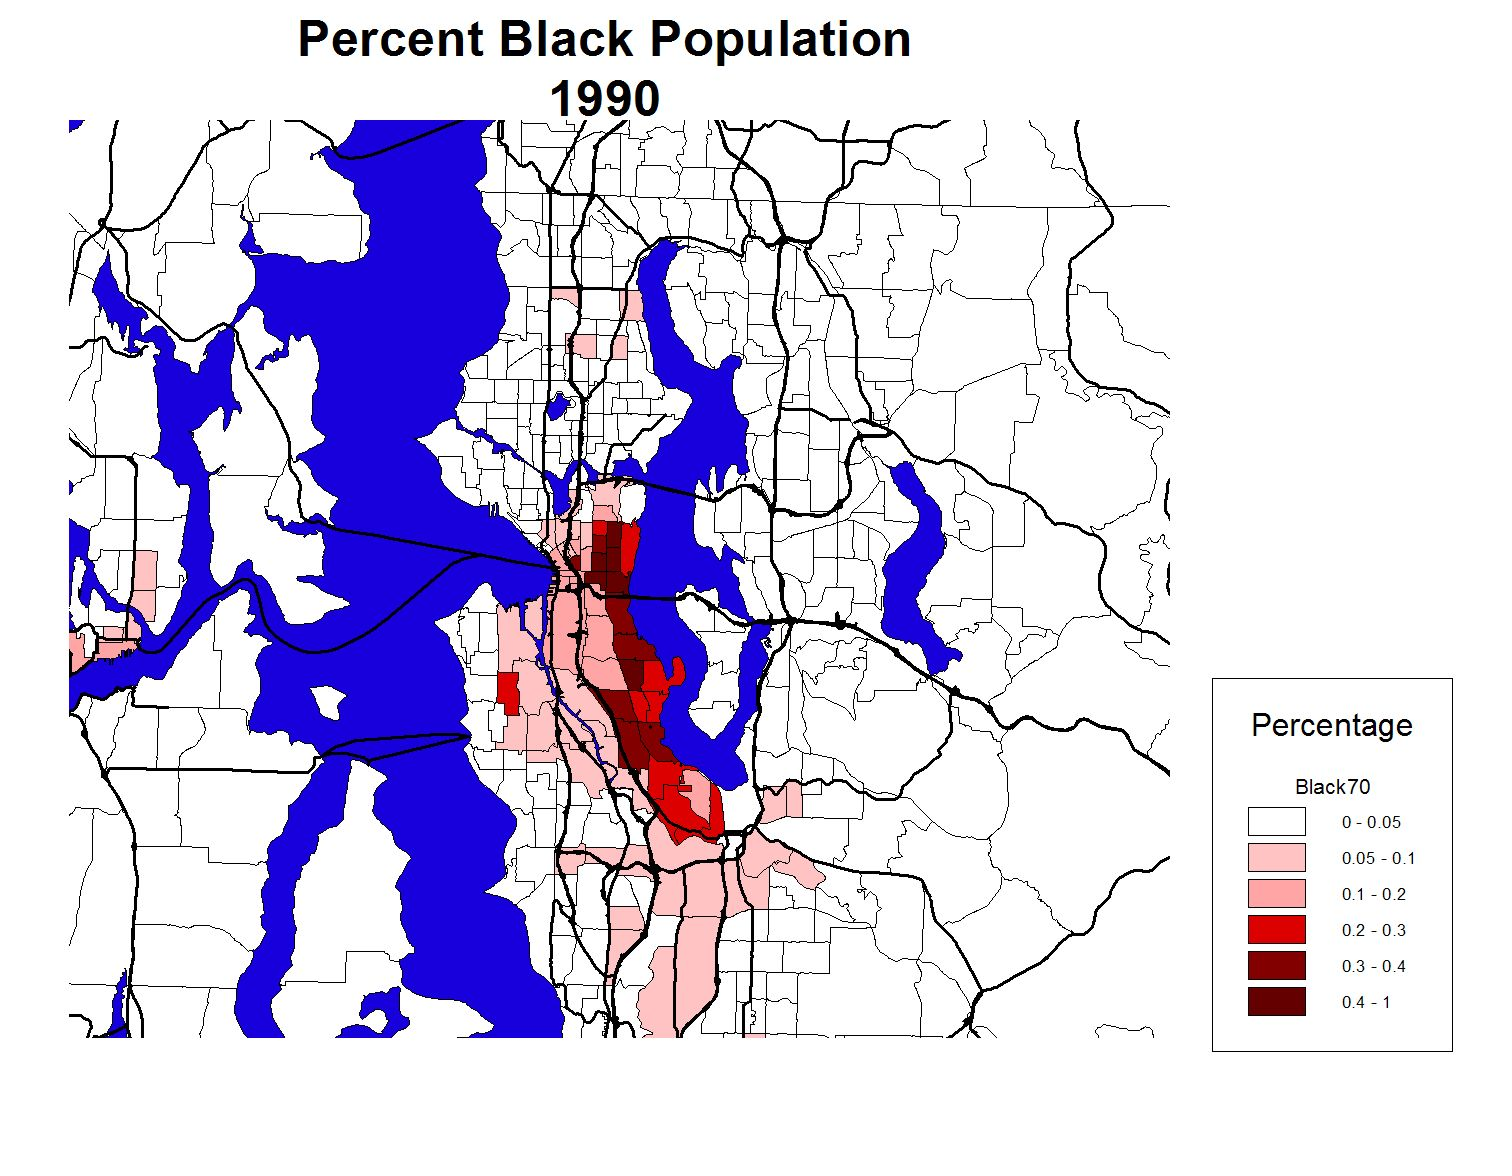
\includegraphics[width=.45\textwidth,height=0.35\textwidth]
 {pctblack1990.jpg} \hspace{1cm}
 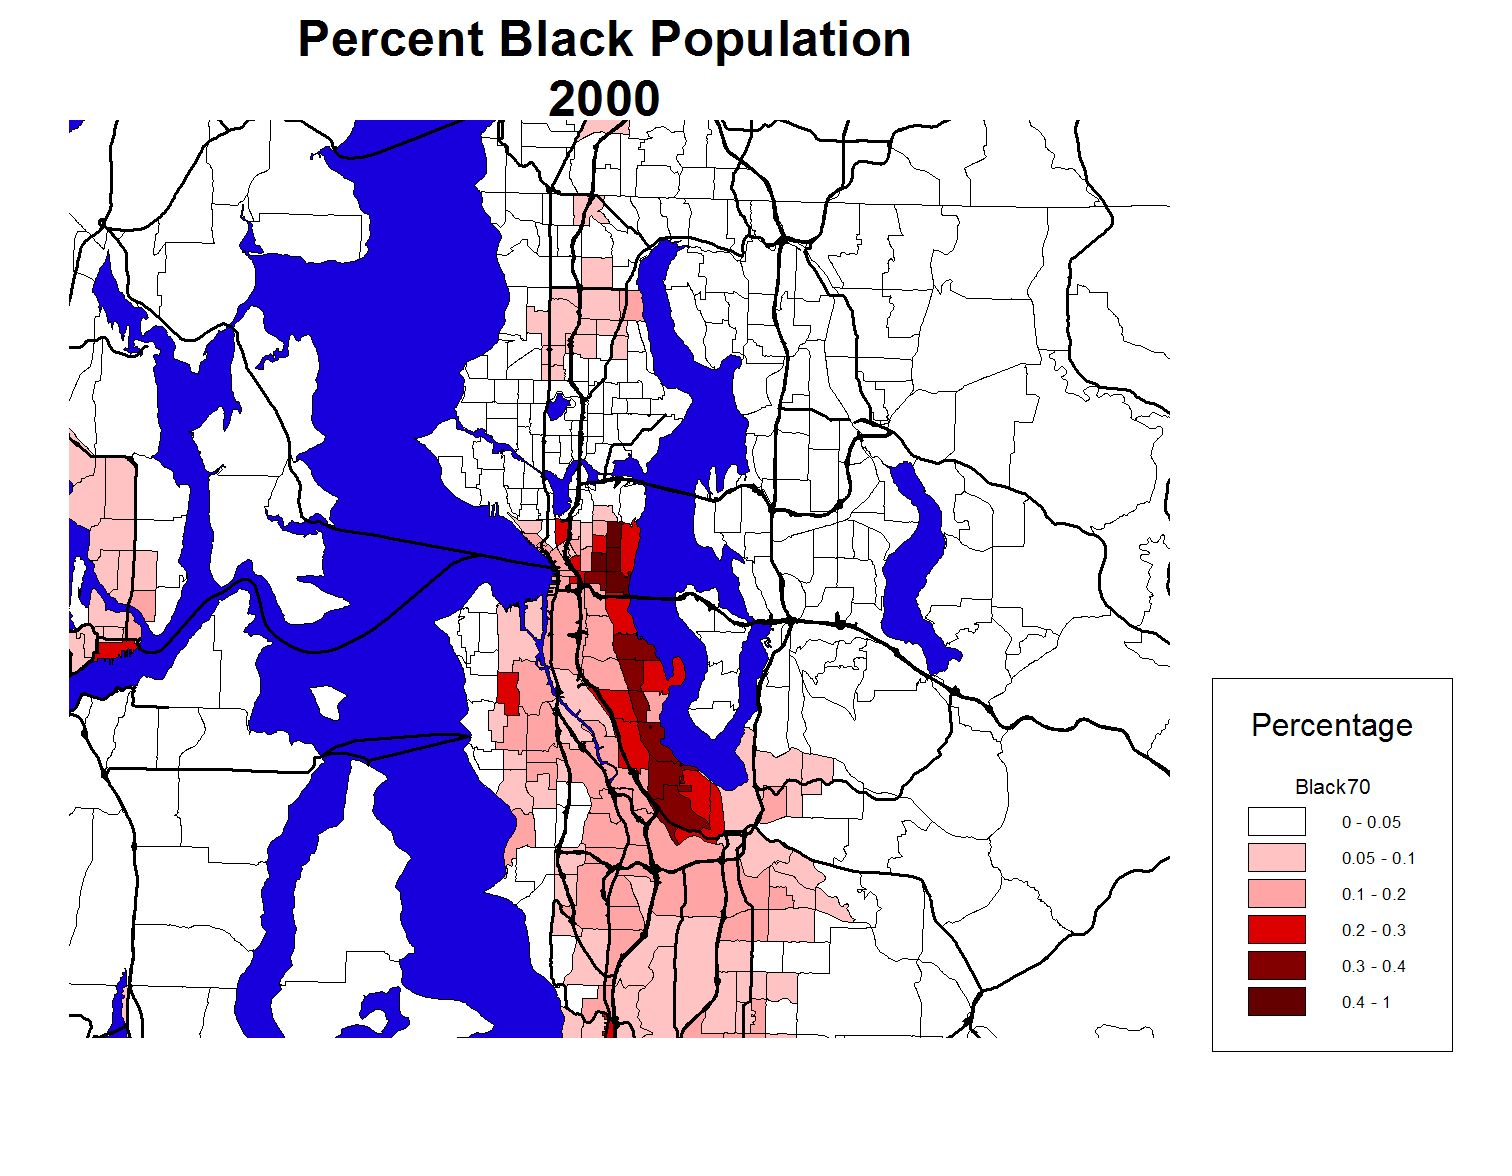
\includegraphics[width=.45\textwidth,height=0.35\textwidth]
 {pctblack2000.jpg}}
\caption{\label{fig:pctblack} Percent Black in Central Seattle}
\end{figure}

The principal objective of this paper is the development of a
methodological approach that facilitates the analysis of
individual choices and the neighborhood dynamics that both result
from and influence these choices, and which can be extended to
address various forms of endogeneity that challenge this research
domain.  In the next section, we describe the modeling framework
to be used in the paper, followed by the specification of the
residential location model and empirical results from its
estimation.  We then turn to problems of endogeneity related to
neighborhood composition, housing prices, housing supply,
transportation, and employment location, and address each by
extending the model system to internalize these sources of
endogeneity.


\section{A Model of Residential Location Choice}

One rapidly growing literature that has approached the analysis of
emergent properties of individual agent choices is the work on
Agent-Based Models (ABMs). Using relatively simple rules to govern
the behavior of agents that are influenced by their immediate
surroundings, ABMs are making significant inroads as a research
method in sociology, political science and economics, among other
fields
\cite{epstein-book-1996,axelrod-book-1997,macy-ars-2002,tesfatsion-handbook-2003}.
Drawing on the emergence of widely available software tools to
develop agent-based models such as Swarm \cite{swarm-web} and
Sugarscape \cite{sugarscape-web}, and stimulated by Schelling's
pioneering work on segregation as an emergent outcome of individual
choices based on weak preferences
\cite{schelling-1969,schelling-1971}, recent work has begun to
develop and test theoretical propositions regarding the emergence of
racial segregation using ABMs 
\cite{bruch-working-2004,fossett-2006,zhang-jms-2004}. The
literature emerging from the ABM approach is principally of a
theoretical nature, with relatively few attempts to empirically test
these models against observed data. Model parameters in the ABM
literature are generally assumed rather than estimated from data,
with some exceptions \cite{bruch-working-2004}.

A different approach to modeling individual actions using discrete
choice models emerged in the 1970's, with the pioneering work of
McFadden on Random Utility Maximization theory
\cite{mcfadden-1974,mcfadden-1981}. This approach derives a model of
the probability of choosing among a set of available alternatives
based on the characteristics of the chooser and the attributes of
the alternative, and proportional to the relative utility that the
alternatives generate for the chooser. Maximum likelihood and
simulated maximum likelihood methods have been developed to estimate
the parameters of these choice models from data on revealed or
stated preferences, using a wide range of structural specifications
(see \cite{train-book-2003}). Early application of these models were
principally in the transportation field, but also included work on
residential location choices
\cite{quigley-eer-1976,lerman-trr-1977,mcfadden-1978}, and, notably,
on residential mobility \cite{clark-vanlierop-1986}.  Rarely has the
research on residential mobility been linked with that on residential
location choice within a single nested choice modeling framework 
\cite{clark-onaka-1985}, but the authors acknowledged limited success 
in modeling the neighborhood choice.  Our focus will be
on the residential location choice rather than on the decision to move,
though in other work we are examining the interdependence
among mobility, residential location and housing tenure \cite{waddell-book-2007}.
In this paper, we draw to some extent on the ABM approach, and more heavily on the
discrete choice modeling approach in the development of the model,
since we need to address agent-level choices and their interaction
within neighborhoods.

\subsection{Study Context and Data}
The setting for the analysis presented in the paper is the
Seattle-Tacoma metropolitan area, locally known as the Central Puget
Sound region.  It contains the Cities of Seattle and Bellevue, and
such notable firms as Amazon.com, Microsoft, Starbucks, and
RealNetworks.  Though a relatively affluent region, with proportions
of poor and of blacks well below national averages, considerable
segregation of poor and blacks still exists, as shown in the Figures
1-2.  One consideration that influences patterns of segregation and
shapes neighborhoods and housing markets is that the region's
topography creates amenity value from waterfront properties and from
views of Mt. Rainier, downtown, lakes and the Puget Sound. These
tend to create a micro-scale variation in income in which expensive
housing is located almost anywhere there is a significant
environmental amenity, leaving the valleys and neighborhoods near
industrial areas to accommodate lower-priced housing.

For use in this study, a very extensive database of parcel data,
employer locations, housing characteristics and prices,
transportation characteristics were available from a substantial
effort to create an integrated database for metropolitan land use
and transportation modeling.  In addition, a 1999 household survey
of household activities and travel was available for use, and
contained information on the household and its members, and their
residential locations, workplaces, and daily activities and travel
patterns over a two day period.  The survey contained
approximately 6,000 households, over 2,400 of which had moved
within the past 5 years.  This sample of recent movers was used to
estimate the residential location choice model described in the
next section.

The level of geographic coding available for the household survey
was a set of point-level coordinates, some of which correspond to
a specific parcel and others of which only fall along the street
segment that contains the residential address.  Given this high
degree of spatial detail, we use a fine-grained mesh to describe
the locations in the region, based on cells of 150 by 150 meters,
and corresponding approximately to a small urban city block (each
cell contains 5.56 acres).  Figure \label{gridmap} provides a
visual representation of these locational units.  For each cell,
information on the housing in the cell and its price are
available, as are characteristics of the physical environment such
as views, steep slopes, or locations in the flood plain.

\begin{figure}[h]
\centerline{
  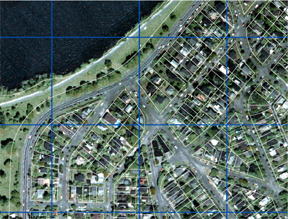
\includegraphics[width=.45\textwidth,height=0.35\textwidth]
 {gridmap-small.png}}
\caption{\label{fig:gridmap} 150 x 150 Meter Grid Cells in Central
Seattle}
\end{figure}

Household agents have characteristics of race, income, size,
presence of children, age of head, number of workers, and number of
vehicles. The initial base year population is derived from census
data using a synthetic population procedure \cite{beckman-1996},
which uses Iterative Proportional Fitting to scale the joint
probability distribution of household characteristics in the Census
Public Use Microdata 5\% Sample to the marginal distributions
available by census tract and block group from Census Summary File
3. A sample of real households is used for model estimation,
generally taken from regional surveys for transportation planning.
These surveys provide detailed geocoding to allow assignment of
locational characteristics to sample households, which is essential
for estimating location choice models.

Due to the importance of access to employment in analyzing household
residential location choices, we developed a detailed inventory of
employment data.  Firms data were available at the level of
individual business establishment, with the sector of the firm, the
number of jobs and the location of the establishment, from the state
Employment Securities Division. We geocoded firms to individual
parcels, when possible, and used imputation algorithms to
probabilistically assign firms to specific parcels within a census
block when an exact parcel match was not made.

Extensive imputation and cleaning of these data were needed to
address gaps and inconsistencies in the data, such as with
tax-exempt properties. The attributes generally include year of
construction, type of development, square footage of building, land
area, land use classification, and land and improvement (building)
values.  These data are then transformed into a grid representation
for model development purposes, combining parcel fragments that fall
into the same grid cell and assigning an overall development type
classification to the cell.  A detailed discussion of the data
integration process is available \cite{waddell-cuspa-2004}.

\subsection{Model Specification}

Let us begin with a simple model of households choosing among
alternative locations in the housing market, which we index by
$i$. For each agent, we assume that each alternative $i$ has
associated with it a utility $U_i$ that can be separated into a
systematic part and a random part:
\begin{equation}
    U_i = u_i + \epsilon_i,
    \label{eq:utility}
\end{equation}
where $u_i = \vk{\beta}\cdot\vk{x}_i$ is a linear-in-parameters
function, $\vk{\beta}$ is a vector of $k$ estimable coefficients,
$\vk{x}_i$ is a vector of observed, exogenous, independent
alternative-specific variables that may be interacted with the
characteristics of the agent making the choice, and $\epsilon_i$
is an unobserved random term. Assuming the unobserved term in
(\ref{eq:utility}) to be distributed with a Gumbel distribution
leads to the familiar multinomial logit model
\cite{mcfadden-1974,mcfadden-1981}:
\begin{equation}
    P_i = \frac{\mathrm{e}^{u_i}}{\sum_j \mathrm{e}^{u_j}},
    \label{eq:mnl}
\end{equation}
where $j$ is an index over all possible alternatives. The
estimable coefficients of (\ref{eq:mnl}), $\vk{\beta}$, are
estimated with the method of maximum likelihood (see for example
\cite{Greene-2002}).

Location alternatives are defined as grid cells that contain at
least one vacant housing unit, and these are randomly sampled in
proportion to the number of housing units.  Estimation of
multinomial logit models using a random sample of alternatives has
been shown to yield consistent estimates of the parameters, though
with some loss of efficiency \cite{ben-akiva-lerman-1987}.

The main working hypotheses that motivate the selection of variables
for empirical testing, drawing widely on the urban sociology and
urban economics literature are as follows, with the resulting
operational variables defined in Table \ref{tab:vardef}:

\begin{itemize}

\item Households prefer to spend a smaller fraction of their
income on housing, after controlling for other characteristics. We
operationalize this as the ratio of the total annualized housing
cost to household income.

\item Households with higher income will prefer housing of higher
quality.  This is operationalized as an interaction of household
income with the building value of the house.

\item Households prefer housing on larger lots, though this
preference is accentuated by having children, and attenuated by
young age.  Several variables operationalize these effects,
including the number of housing units in the cell under
consideration, the number of housing units within 600 meters
(roughly 1/3 mile), and the interaction of a dummy for a household
with children and a dummy for having a household head less than 40
years old.

\item Households prefer to reduce commuting costs to work by auto
mode or by transit.  These are operationalized as the expected
travel utility from a residence location to workplaces, weighted
by the trip-making frequencies to work from that location.

\item Households may prefer to avoid locations on an arterial
street.  We measure the presence of an arterial adjacent to each
grid cell.

\item Households tend to segregate by income.  We measure three
interaction terms, reflecting the income tercile of the household
making a location choice and the percent of households within 600
meters that are of the same tercile.

\item Households tend to segregate by race.  We measure the
interaction of a dummy for minority head of household with percent
minority within 600 meters, and an interaction between a dummy for
white households with the percent minority within 600 meters.  Note
that this does not address whether the segregation occurs entirely by
the choice of the locating households, or as a result of discrimination
in the housing market, or some combination thereof.

\item Households at different stages of the life cycle may reveal
differing locational preferences. Household size and age of head
are used to stratify the model estimation and allow estimation of
different preference structures across the life cycle.

\end{itemize}


\subsection{Estimation Results}
Model estimation results using a sample of 2,364 households who
moved between 1995 and 2000 are given in Table \ref{tab:hlc}.

\begin{table}[h]
\caption{Variables Used in Household Location Choice Model, Puget
Sound Region} \label{tab:vardef} \centering
\begin{tabular}{ll}
\hline\hline
BCOS\_IN & Annualized Cost of Housing / Household Income \\
BDUR\_C & Dwelling Units in Cell * Has Children Dummy \\
BART & Close to Arterial Dummy \\
BINCIVAL & Income * Improvement Value per Unit \\
BLDUW & Log of Dwelling Units within 600 Meters \\
BPHIW\_H & High Income Dummy * Pct High Income in 600 Meters \\
BPMIW\_M & Middle Income Dummy * Pct Middle Income within 600
Meters \\
BPLIW\_L & Low Income Dummy * Pct Low Income Within 600 Meters
\\
BPMNWMJ & Minority Dummy * Pct Minority Within 600 Meters
\\
BPMNWMN & White Dummy * Pct Minority Within 600 Meters \\
BSAGEFAZ & Number of Households in FAZ of Same Age Category as
Household \\
SSIZFAZ & Number of Households in FAZ of Same Size Category as
Household \\
BYH\_HDR & Young Household Head (< 40) * High Density Residential
\\
YH\_M & Young Household Dummy * Mixed Use \\
BHBWUSO & Utility of Travel to Work by Auto \\
BHBWUTW & Utility of Travel to Work by Transit \\

\hline
\end{tabular}
\end{table}

The cost to income ratio provides an interaction that captures
price effects on location choice.  It is expected have a negative
sign, meaning that households prefer spending a smaller fraction
of their income on housing if presented with two alternatives that
are the same on all other measured characteristics except cost.
The results are all negative, and significant for all except young
single-person and 3+ person households.

The interaction of income of household with the percentage of
households of the same income tercile within the area within
walking distance (600 meters) are significant and positive for
only 6 of the 18 parameters estimated (3 parameters for 6 types of
households), with the strongest positive effects for younger
households with 3 or more persons.

The interaction between minority households and the percent
minority within walking distance was positive for all but young
one-person households, and significant for all households with at
least 2 persons.  White households had negative and significant
coefficients on the percentage minority within walking distance in
all six household types.

Age clustering was tested with the same age in FAZ (a larger
neighborhood geography used in the region) but found to be
significant only for young singles, not an entirely surprising
result.  Younger households and those without children also showed
quite different preferences for urbanization, as measured by transit
utility and density of housing in a cell, with a greater affinity to
areas with high transit utility and higher density.

\clearpage
\begin{table}[h]
\caption{Estimation Results for Household Location Choice Model,
Puget Sound Region} \label{tab:hlc} \centering
\begin{tabular}{lrr|rr|rr}
\\
Age 40 or Less  &   \multicolumn{2}{c}{1 Person}  &
\multicolumn{2}{c}{2 Person}   &   \multicolumn{2}{c}{3 or More Persons}    \\
\hline\hline & beta & b./std. err & beta & b./std. err & beta &
b./std. err \\
BCOS\_IN &   -0.2557 &   -1.63   &   -1.7230 &   -4.74   &   -0.1572 &   -1.20   \\
BDUR\_C  &       &       &   -0.0122 &   -2.24   &   -0.0111 &   -5.14   \\
BART    &   0.2072  &   1.44    &   0.0684  &   0.49    &   -0.1166 &   -1.00   \\
BINCIVAL    &   0.0000  &   1.28    &   0.0000  &   5.54    &   0.0000  &   6.36    \\
BLDUW   &   0.3763  &   3.18    &   0.2172  &   2.08    &   0.2857  &   4.16    \\
BPHIW\_H &   0.0381  &   2.66    &   0.0080  &   0.81    &   0.0144  &   2.07    \\
BPMIW\_M &   0.0164  &   1.59    &   0.0166  &   1.76    &   0.0267  &   4.19    \\
BPLIW\_L &   0.0214  &   2.50    &   -0.0016 &   -0.14   &   0.0185  &   2.34    \\
BPMNWMJ &   -0.0021 &   -0.18   &   0.0312  &   2.50    &   0.0225  &   2.39    \\
BPMNWMN &   -0.0152 &   -2.58   &   -0.0188 &   -3.12   &   -0.0182 &   -3.80   \\
BSAGEFAZ    &   0.0005  &   3.66    &   0.0002  &   1.67    &   0.0000  &   0.29    \\
SSIZFAZ &   -0.0001 &   -1.68   &   0.0000  &   -0.27   &   0.0002  &   1.87    \\
BYH\_HDR &   0.4440  &   1.53    &   0.5632  &   2.29    &   0.3565  &   1.98    \\
YH\_M    &   0.4582  &   1.46    &   0.7549  &   2.79    &   0.6555  &   2.88    \\
BHBWUSO &   1.2211  &   0.87    &   1.0097  &   0.83    &   2.8577  &   3.74    \\
BHBWUTW &   13.1195 &   1.61    &   14.2051 &   1.88    &   -22.7206    &   -3.63   \\
\hline \\
Age Over 40 & \multicolumn{2}{c}{1 Person}   &
\multicolumn{2}{c}{2 Person}   &     \multicolumn{2}{c}{3 or More Persons}    \\
\hline
BCOS\_IN &   -0.9677 &   -4.68   &   -0.8034 &   -2.97   &   -1.1394 &   -2.50   \\
BDUR\_C  &       &       &       &       &   -0.0150 &   -3.58   \\
BART    &   0.2878  &   2.16    &   0.1349  &   0.97    &   0.1930  &   1.13    \\
BINCIVAL    &   0.0000  &   2.93    &   0.0000  &   7.02    &   0.0000  &   6.08    \\
BLDUW   &   0.2436  &   2.37    &   0.1162  &   1.39    &   0.2166  &   2.21    \\
BPHIW\_H &   0.0168  &   1.11    &   0.0139  &   1.71    &   0.0108  &   1.32    \\
BPMIW\_M &   0.0096  &   0.93    &   0.0132  &   1.52    &   0.0123  &   1.27    \\
BPLIW\_L &   0.0165  &   2.14    &   0.0029  &   0.30    &   -0.0019 &   -0.13   \\
BPMNWMJ &   0.0117  &   0.68    &   0.0590  &   3.50    &   0.0405  &   2.68    \\
BPMNWMN &   -0.0255 &   -4.22   &   -0.0117 &   -2.03   &   -0.0313 &   -3.85   \\
BSAGEFAZ    &   0.0002  &   1.37    &   0.0002  &   0.79    &   -0.0002 &   -0.87   \\
SSIZFAZ &   0.0000  &   -0.50   &   -0.0001 &   -0.45   &   0.0004  &   2.10    \\
BHBWUSO &   2.7715  &   2.28    &   3.3305  &   3.42    &   1.7744  &   1.55    \\
BHBWUTW &   12.7920 &   1.58    &   -9.5427 &   -1.28   & -13.4521 &   -1.38 \\
\hline\hline

\end{tabular}

\end{table}
\clearpage

The interactions of household characteristics and social
composition of neighborhoods, measured at scales from the grid
cell, to walking distance, to larger FAZ geographies, measure the
degree to which neighborhood composition influences individual
choice of residence location.  These results are informative regarding 
individual household
preferences for residential location, incorporating life cycle and
income of the household and their interaction with exogenous
effects from housing supply, housing prices, neighborhood ethnic
and income composition, and commuting access.  Unfortunately, none
of the exogenous factors considered, are, in fact, exogenous.  In the
remainder of this paper, we
develop an approach to embed the residential location choice
model we have estimated within an interacting system of models
in order to better account for these sources of endogeneity.  It is
of course important to consider that neighborhood change occurs
over periods of many years, and the choices of individual households
in a single housing location choice are made within much briefer
time periods.  To address these modeling requirements, we have 
developed UrbanSim, an Open Source microsimulation system
\cite{waddell-env-and-planning-2000,waddell-japa-2002,waddell-tra-2007,
sevcikova-trb-2007}.

\section{Extensions to Address Endogeneity}

If we cannot assume that several of the variables on the right hand
side of the residential location choice model are truly exogenous
over periods of a decade or longer, we need to model the
interactions between households making location choices in the
housing market, housing suppliers building new housing, and firms
choosing where to place jobs.  The interactions among these choice
processes produce two systemic outcomes: housing prices and an
allocation of households that reconciles demand and supply among
neighborhoods, and accessibility to jobs. Each of these choice
processes and their systemic outcomes should be represented by
additional models, linked together to simulate dynamic outcomes, in
order to address this endogeneity bias.  In order to handle the
interactions among several choice models, we implement the model
within a simulation framework designed for this purpose.

\subsection{UrbanSim: A System for Interacting Urban Models}

UrbanSim is an open-source simulation system developed over the
past several years to support the analysis of individual-level
models related to urban dynamics
\cite{waddell-japa-2002,waddell-nse-2003}. We use this framework
to simulate the residential location choice model as reported in
the preceding section, and to interface this with models of firm
location choice, real estate development for housing and
non-residential space, real estate prices, and the interaction of
the urban system with the transportation system, which reconciles
the demand for travel for commuting to work and to other
activities with available transportation system capacity. Figure
\ref{fig:urbansim} portrays the key model components and their
sequence of operation within a time-step of one year. Processing
an agent-level model of this type efficiently, when the number of
agents can be in the millions and the number of alternatives can
be in the hundreds of thousands, required an innovative software
design, and we found existing Agent-Based Modeling software
platforms insufficient to handle this task \cite{noth-ceus-2003}.

UrbanSim has been applied in several metropolitan regions,
including Eugene-Springfield, Oregon, Honolulu, Hawaii, Houston,
Texas, Salt Lake City, Utah \cite{waddell-tra-2007}, Seattle, 
Washington, and Paris, France \cite{depalma-jue-2007}, and has been
validated longitudinally by comparing 15 years of path-dependent
simulation to observed outcomes 
\cite{waddell-japa-2002,sevcikova-trb-2007}.  Several
more metropolitan areas are in the early stages of applying the
model system in the U.S., such as Denver, Colorado and Detroit,
Michigan, and abroad, including Amsterdam, the Netherlands, 
 and Z\"{u}rich, Switzerland.

\begin{figure}[t]
\begin{center}
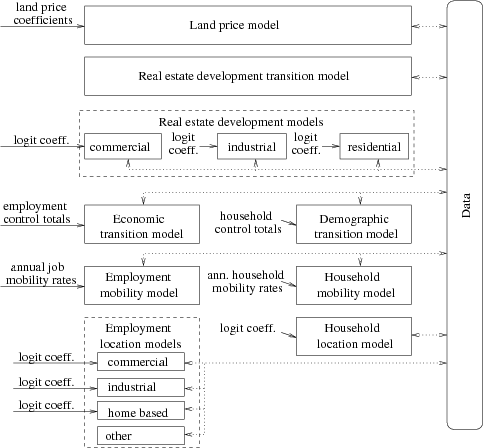
\includegraphics[scale=0.8]{UrbanSim_with_par.png}
\caption{\label{fig:urbansim} \small UrbanSim models in order of
their runs
  (from top to bottom). The solid arrows show external input parameters. The
  dashed arrows mark the data flow: data are input to the different models,
  and these in turn modify the data.}
\end{center}
\end{figure}



\begin{figure}[h]
\center
 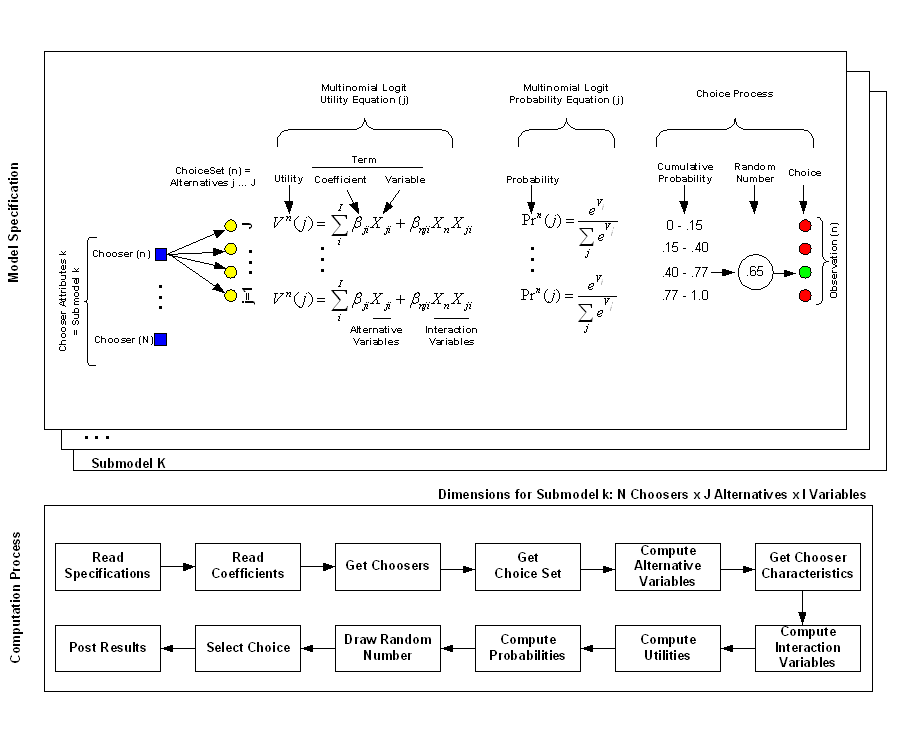
\includegraphics[width=6.5in]
 {ChoiceProcess.png}
\caption{Choice Process in UrbanSim Location Choice Models}
\label{fig:choiceprocess}
\end{figure}

For each model component within the UrbanSim model system, the
choice process proceeds as shown in Figure
\ref{fig:choiceprocess}. The first steps of the model read the
relevant model specifications and data.  Then a choice set is
constructed for each chooser.  Currently this is done using random
sampling of alternatives, where alternatives are grid cells of 150
meters by 150 meters, and the cells are weighted by the number of
locational opportunities in them (vacant housing for the
residential location choice model).  Note that this sampling
method has been shown to generate consistent, though not
efficient, estimates of model parameters
\cite{ben-akiva-lerman-1987}.

Once the choosers (movers or new households) are selected and the
choice sets of alternative locations sampled, the relevant
variables used in the utility function are computed.  For
efficiency, this proceeds by computing characteristics of
alternatives first for all alternatives in the universe, then
computing interaction terms for only the set of choosers and their
sampled locations.  After this, the logit calculations predict
probabilities for all the available choices in the choice set for
each chooser.  Finally, the process makes a selection by drawing a
random number, comparing it to the cumulative distribution of the
predicted alternatives, and selecting the choice which the random
draw falls within.  At this point the choice is committed for the
chooser, and the number of available housing units is reduced by
one to reflect that the unit is no longer vacant.

Space constraints prevent a full reporting of the specification and
estimation results for each of the component models, or the results
of extensive sensitivity testing of the combined model system, these
results are available elsewhere \cite{waddell-cuspa-2004}.  We turn
next to extensions of the model system to address endogeneity due to 
housing prices and neighborhood sorting.


\subsection{Endogenous Market Clearing and Prices}

A major endogeneity issue arises in the context of location
choice, due to the need to reconcile the choices made by locating
agents with the fixed available supply of real estate at those
locations. We shall refer to this in general as a \emph{market
clearing} process, but only in the limited sense that we impose
the accounting constraint that once a location (housing unit) is
chosen by an agent, it is occupied and not available to another
agent until it is vacated by the first.  This means that there
will often be a scarcity of housing at more desirable locations,
and there must be some means to ration the scarce housing among
the agents that wish to locate in them. The assumption of a fixed
supply (stock) of housing in the short-run is equivalent to
assuming that if a household is looking for a house this month,
they cannot contract to have a house built and made available for
them next month.  The time frame for housing supply is
considerably longer than the time scale for residential location
choice, due to the time-consuming processes that real estate
developers must undertake once they decide to develop a property.

The process currently used in UrbanSim, shown in Figure
\ref{fig:choiceprocess}, simulates the market clearing constraint
by assuming that the scarcity of housing at any given location is
rationed according to a randomized order, first-come-first-served
process, essentially representing a lottery for the available
houses. Experience confirms that there is a strong degree of
random, but sequential, dependence in the way the housing market
works: if person A arrives first and makes a successful bid on a
house, it is not available to person B, even if the latter would
be willing to pay more.

A visual example of the current algorithm makes the process
clearer. Let us simplify the situation to one in which there are
16 neighborhoods, arranged in a rectangular grid.  Assume that
they have 10 houses in each and that there are exactly 160
identical households looking for housing.  Assume further that the
attractiveness of the neighborhoods varies in a systematic way:
cells in the corners have the least attractiveness (1), those on
the edge and not in the corners have an attractiveness of (2), and
those in the center have the highest attractiveness (3).  Note
that the utility is defined as the exponentiated value of these
attractiveness terms (using the multinomial logit model), and it
is the relative utility that directly influences choice
probabilities. Figure \ref{fig:grid1} shows the attractiveness
(a), sums of the individual choice probabilities (b), the count of
choices made by this sample of 160 households on this particular
draw of random numbers \footnote{Note that with a relatively small
number of observations the sum of the choice probabilities differs
significantly from the choice counts due to simulation randomness.
This simulation error diminishes as the number of observations
increases.} (c), and the excess demand in those cells that the
counts exceed housing supply (d).  The excess demand would be the
number of households forced to make a suboptimal choice from the
remaining available housing, and this would proceed until all
households are placed, provided that there is available housing.
In this example, it would mean that each cell would end up with 10
households, though many would have preferred to locate in the
center cells.

This algorithm for market clearing is at the opposite end of the
spectrum from the algorithm assumed in economic models, where prices
would fully adjust to clear the market.  Real markets are more
likely to involve a role both for prices and for some form of
non-price rationing. It is implausible to assume that all
households participate in a single massive auction, and each obtains
the house they most prefer, subject to budget constraints, in a
competitive bidding process. It is more likely that the random
arrival and bidding processes are both facets of the actual
operation of the market.

To modify the algorithm shown in Figure \ref{fig:choiceprocess} to
reflect the standard economic assumption that prices clear the
market, we could simulate the role of a 'landlord' agent in each
neighborhood who monitors market conditions and attempts to
maximize profit by adjusting prices. Depending on how elastic the
demand is, due to substitution possibilities among alternative
neighborhoods, a landlord would increase prices in the presence of
multiple offers in order to increase profit, and lower prices if
the number of offers falls well below the number of housing units
available in the neighborhood.  This would be implemented as an
iterative loop at the choice stage, with landlords updating prices
to improve profits, and households altering their choices in the
face of modified prices.  Notice that both of these agent
responses are consistent with expected behavior, intuitively and
theoretically, and both work to restore balance between demand and
supply.  The revised algorithm is shown in Figure
\ref{fig:choiceprocess2}.


\begin{figure}[h]
\centerline{
 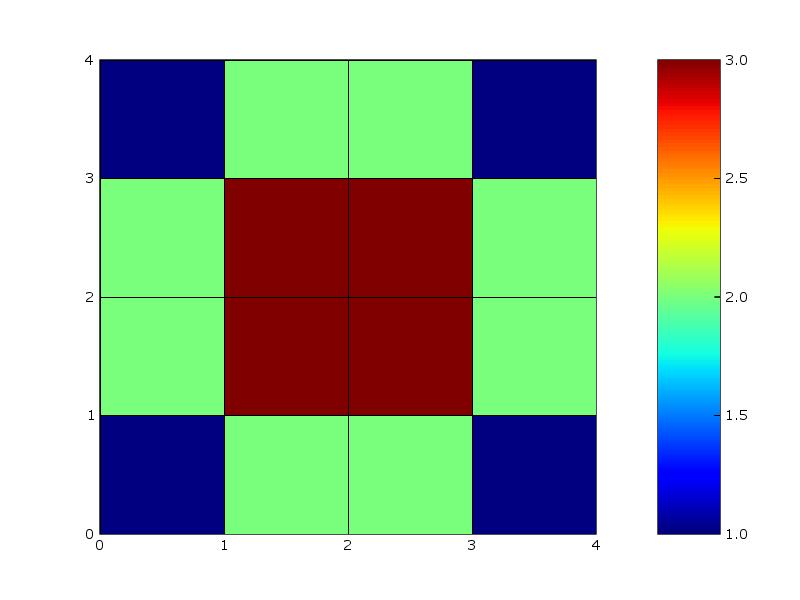
\includegraphics[width=.25\textwidth,height=0.2\textwidth]
 {example_grid_util.png} \hspace{1cm}
 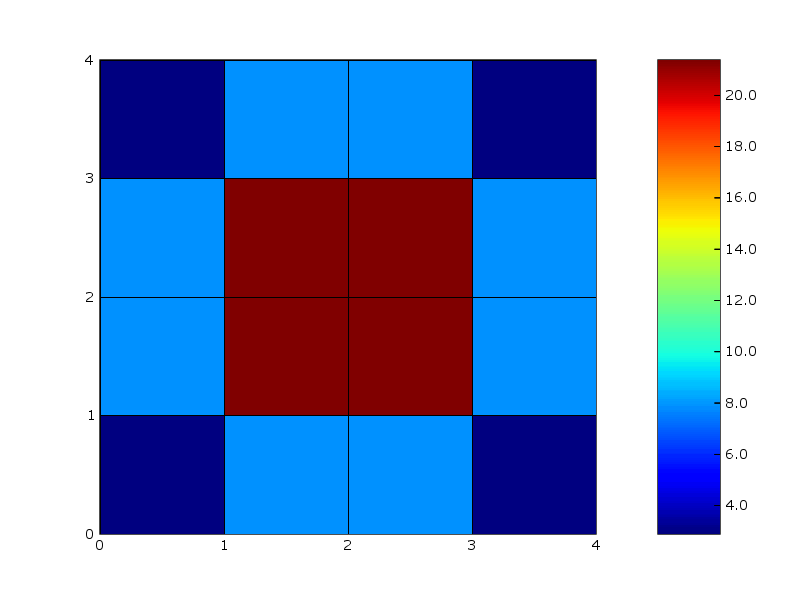
\includegraphics[width=.25\textwidth,height=0.2\textwidth]
 {example_grid_prob.png}}
\end{figure}

\begin{figure}[h]
\centerline{
 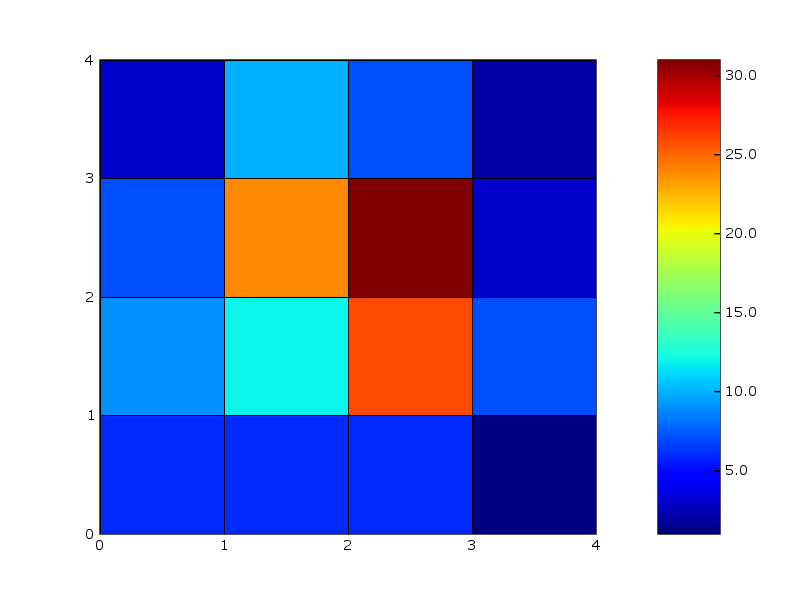
\includegraphics[width=.25\textwidth,height=0.2\textwidth]
 {example_grid_count.png} \hspace{1cm}
 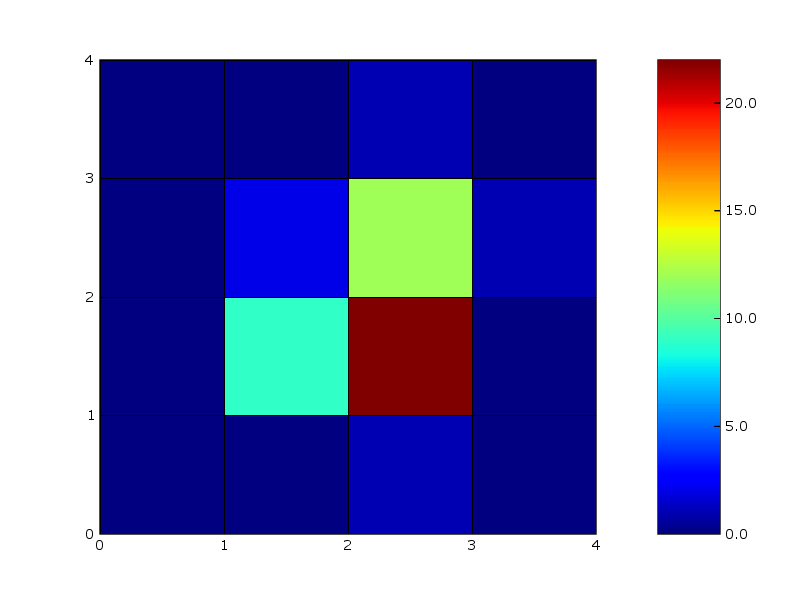
\includegraphics[width=.25\textwidth,height=0.2\textwidth]
 {example_grid_excess.png}}
\caption{\label{fig:grid1} Choice Model Predictions With Limited
Housing}

\begin{tabbing}
------- \= ------------------------------------------------------------ \= \kill
\> (a) Attractiveness (log(Utilities))  \> (b) Sum of
Probabilities \\  \> (c) Choices (among 160 choosers) \> (d)
Excess Demand
\end{tabbing}
\end{figure}



\begin{figure}[h]
\center
 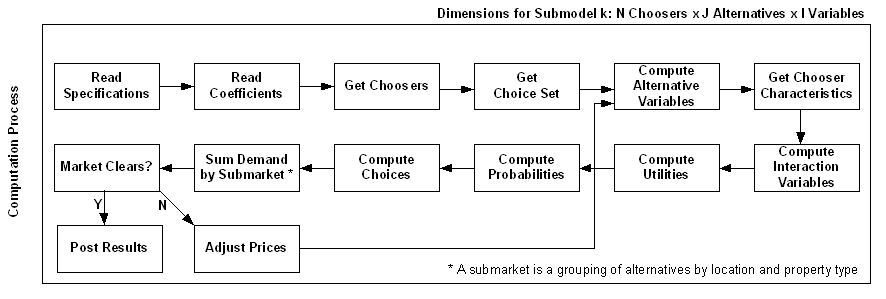
\includegraphics[width=6.5in]
 {ChoiceProcessWithPriceAdjustment.png}
\caption{Choice Process in UrbanSim Location Choice Models}
\label{fig:choiceprocess2}
\end{figure}


A more realistic alternative would be to add a method to the
algorithm to allow the relative weight of the price adjustment
process and the lottery process to vary depending on parameters
derived from model calibration against observed data.  It should be
possible to avoid imposing an arbitrary assumption that only the
price mechanism or only the lottery mechanism are at work, and it
should also be possible to learn the mixture of these processes by
examining observed data. This modification will require a
re-specification of the logit model to include both a constraint and
a price effect, and adjusting the coefficients of the model to
distinguish between constraint effects and preferences.  A new
algorithm that uses this approach has been developed in
\cite{depalma-jue-2007}.


\subsection{Endogenous Neighborhood Composition}
The literature on residential location choice contains several
streams of research on aspects that link the choices made by
individual households to emergent spatial patterns. If the social
composition of a neighborhood selection is valued by a locating
household, and the outcome of their residential location choice
changes the social composition of the neighborhood they locate in,
then the individual choice process and the neighborhood composition
are endogenous.

One approach to analyzing this endogeneity was developed by Thomas
Schelling \cite{schelling-1969,schelling-1971,schelling-1978}. This
approach and its extensions simulates the relocation choices of
individual agents based on their satisfaction with the social
composition in their localized neighborhood. Schelling's early model
of residential segregation has inspired considerable extension in
the multi-agent simulation literature.  Its attractiveness, and the
attraction of more recent work on this approach, derive in no small
measure from its transparent simplicity.  The utility function is
essentially due to a single factor, there are no costs to changing
locations, and no constraints on doing so.

Adding complexity to the utility function, and imposing accounting
constraints on housing supply and a market clearing process as
discussed in the preceding section would makes this modelling
approach considerably less elegant, and possibly less informative.
More problematic from a practical perspective is that there is
considerable computing overhead to processing all agent choices as
localized interactions of agents.  Scaling the model from a small
hypothetical situation to modelling metropolitan regions with
millions of agents would not be practical on generally-available
computers. Last, it seems likely that localized interactions are
insufficient to capture the rich variety of information flow that
informs agent choices. Information about housing market
opportunities for example may come from a newspaper or web site,
personal experience such as seeing a for sale or rent sign while
travelling through a neighborhood, information from a social
network, or from a real estate broker.

The approach used in UrbanSim to model endogenous neighborhood
composition is to include in the utility function interaction terms
between household characteristics and social characteristics of the
location.  The household characteristics used in UrbanSim include
race, household income, age of head, presence of children, number of
persons, number of workers, and number of vehicles.  Since the model
uses full enumeration of the households, generating compositional
measures using these characteristics is straightforward. What is
less straightforward is the choice of which interaction terms to
include in the utility function, and what spatial frames to use for
the measurement of the social composition effect.  To date, only a
small subset of the possible interaction terms have been tested in
the model system, though the framework and data exist to test
others.

The treatment of endogenous neighborhood sorting has been addressed
in the economics literature, using an approach developed by Berry,
Levinsohn and Pakes to model the automobile market
\cite{berry-econometrica-1995,berry-cowles-2003}. This approach has
recently been adapted to the housing market and treatment of
endogenous sorting
\cite{bajari-kahn-stanford-working-papers-2002,bayer-mcmillan-rueben-2003},
but requires even more extensive data than used in this paper, and
imposes strong assumptions about the operation and structure of the
market, and the nature of market equilibrium.  

The spatial frame for measuring effects is challenging because of
the theoretical and empirical limitations in our understanding of
neighborhoods and neighborhood effects.  It is clear that defining
neighborhoods is a problematic exercise, since residents often
disagree about or do not know the boundaries of their neighborhoods,
and that the frames of reference differ depending on the issue at
hand: for example shopping for groceries or choosing a high school.
Moreover, the use of fixed-boundary neighborhoods can give rise to
boundary problems and to potential for the Modifiable Aerial Unit
Problem (MAUP) \cite{openshaw-taylor-1981}. For these reasons, we
have opted to make the selection of spatial frames of reference as
flexible as possible, using grid cells or parcels as the low-level
spatial building block.


\section{Conclusions}

Household residential location choices are instrumental in
determining the dynamics of neighborhoods, and in turn are strongly
affected by those same neighborhood dynamics.  This endogeneity
poses significant challenges to research that seeks to improve
understanding or inform policy regarding issues such as neighborhood
decline, poverty concentration, or racial segregation.  We have
described a model application that attempts to address some of the
main sources of endogeneity, by:

\begin{itemize}
\item representing the bi-directional influence of individual choices of
residential location and emergent neighborhood social and economic
composition;

\item representing the interdependence between residential location
choices and housing prices; and

\item representing the interactions among household location, firm
location, and real estate development.

\end{itemize}

The model system has been estimated and applied in the Puget Sound region 
of Washington, and in a variety of other metropolitan areas in the U.S. and
abroad.  While the sources of endogeneity arising from neighborhood 
composition, housing prices, housing supply, and employment location have
all been addressed in the model system specification, more remains to be
done in examining the nature of the interdependencies, and fully
validating the model system and its interactions and to address other
sources of endogeneity or possible bias, such as from the interdependence of
residence and workplace location.

Current research on developing the modeling approach described in the paper
is focused on developing it for use in
evaluating alternative policy interventions, including
transportation investments, land use regulations and housing
policies.  The platform it is implemented in has been released on
the web as open source software as part of a collaborative 
research effort, the Open Platform for Urban Simulation
(OPUS)\cite{waddell-opus-2005}.  It contains a modular approach to building
models and systems of interacting models, focusing particularly on choice models.
The system also incorporates facilities for estimation of model parameters, in
addition to simulation and visualization of results.  Our motivation
for developing this platform and sharing it as Open Source software on the Internet is
that the absence of computational infrastructure presents a significant obstacle to 
progress in understanding urban neighborhood dynamics, their implications, and the 
potential effects of alternative interventions.  We hope to extend this 
platform and to encourage others to contribute to its development as a tool for 
research and policy analysis.  A framework for incorporating user-contributed 
'packages' is being incorporated into the system to facilitate this.  Currently a
series of indicators of segregation are being incorporated, along with measures
of inequality to assess the distributional consequences of alternative policies.

Other related research has been developing a new approach to addressing the 
interdependence among household choice dimensions, such as residential and workplace
choices \cite{waddell-trr-2007}, or residential location and mode choice to work 
\cite{pinjari-transportation-2007}.
New modeling methods, coupled with theoretical development in the behavior of households
in residential and related choices, offer considerable potential to generate new insights into 
long-standing problems of understanding location choices and neighborhood composition.


\vspace{1cm} {\bf \large Acknowledgments}

%\section{Acknowledgments}
This research has been funded in part by National Science Foundation
Grants EIA-0121326 and IIS-0534094, by EPA Grant R831837, 
and by the Puget Sound Regional Council.

\vspace{1cm}

\bibliography{urbansim}
\bibliographystyle{plain}
\end{document}
